% Created by tikzDevice version 0.12.3.1 on 2022-05-12 12:25:06
% !TEX encoding = UTF-8 Unicode
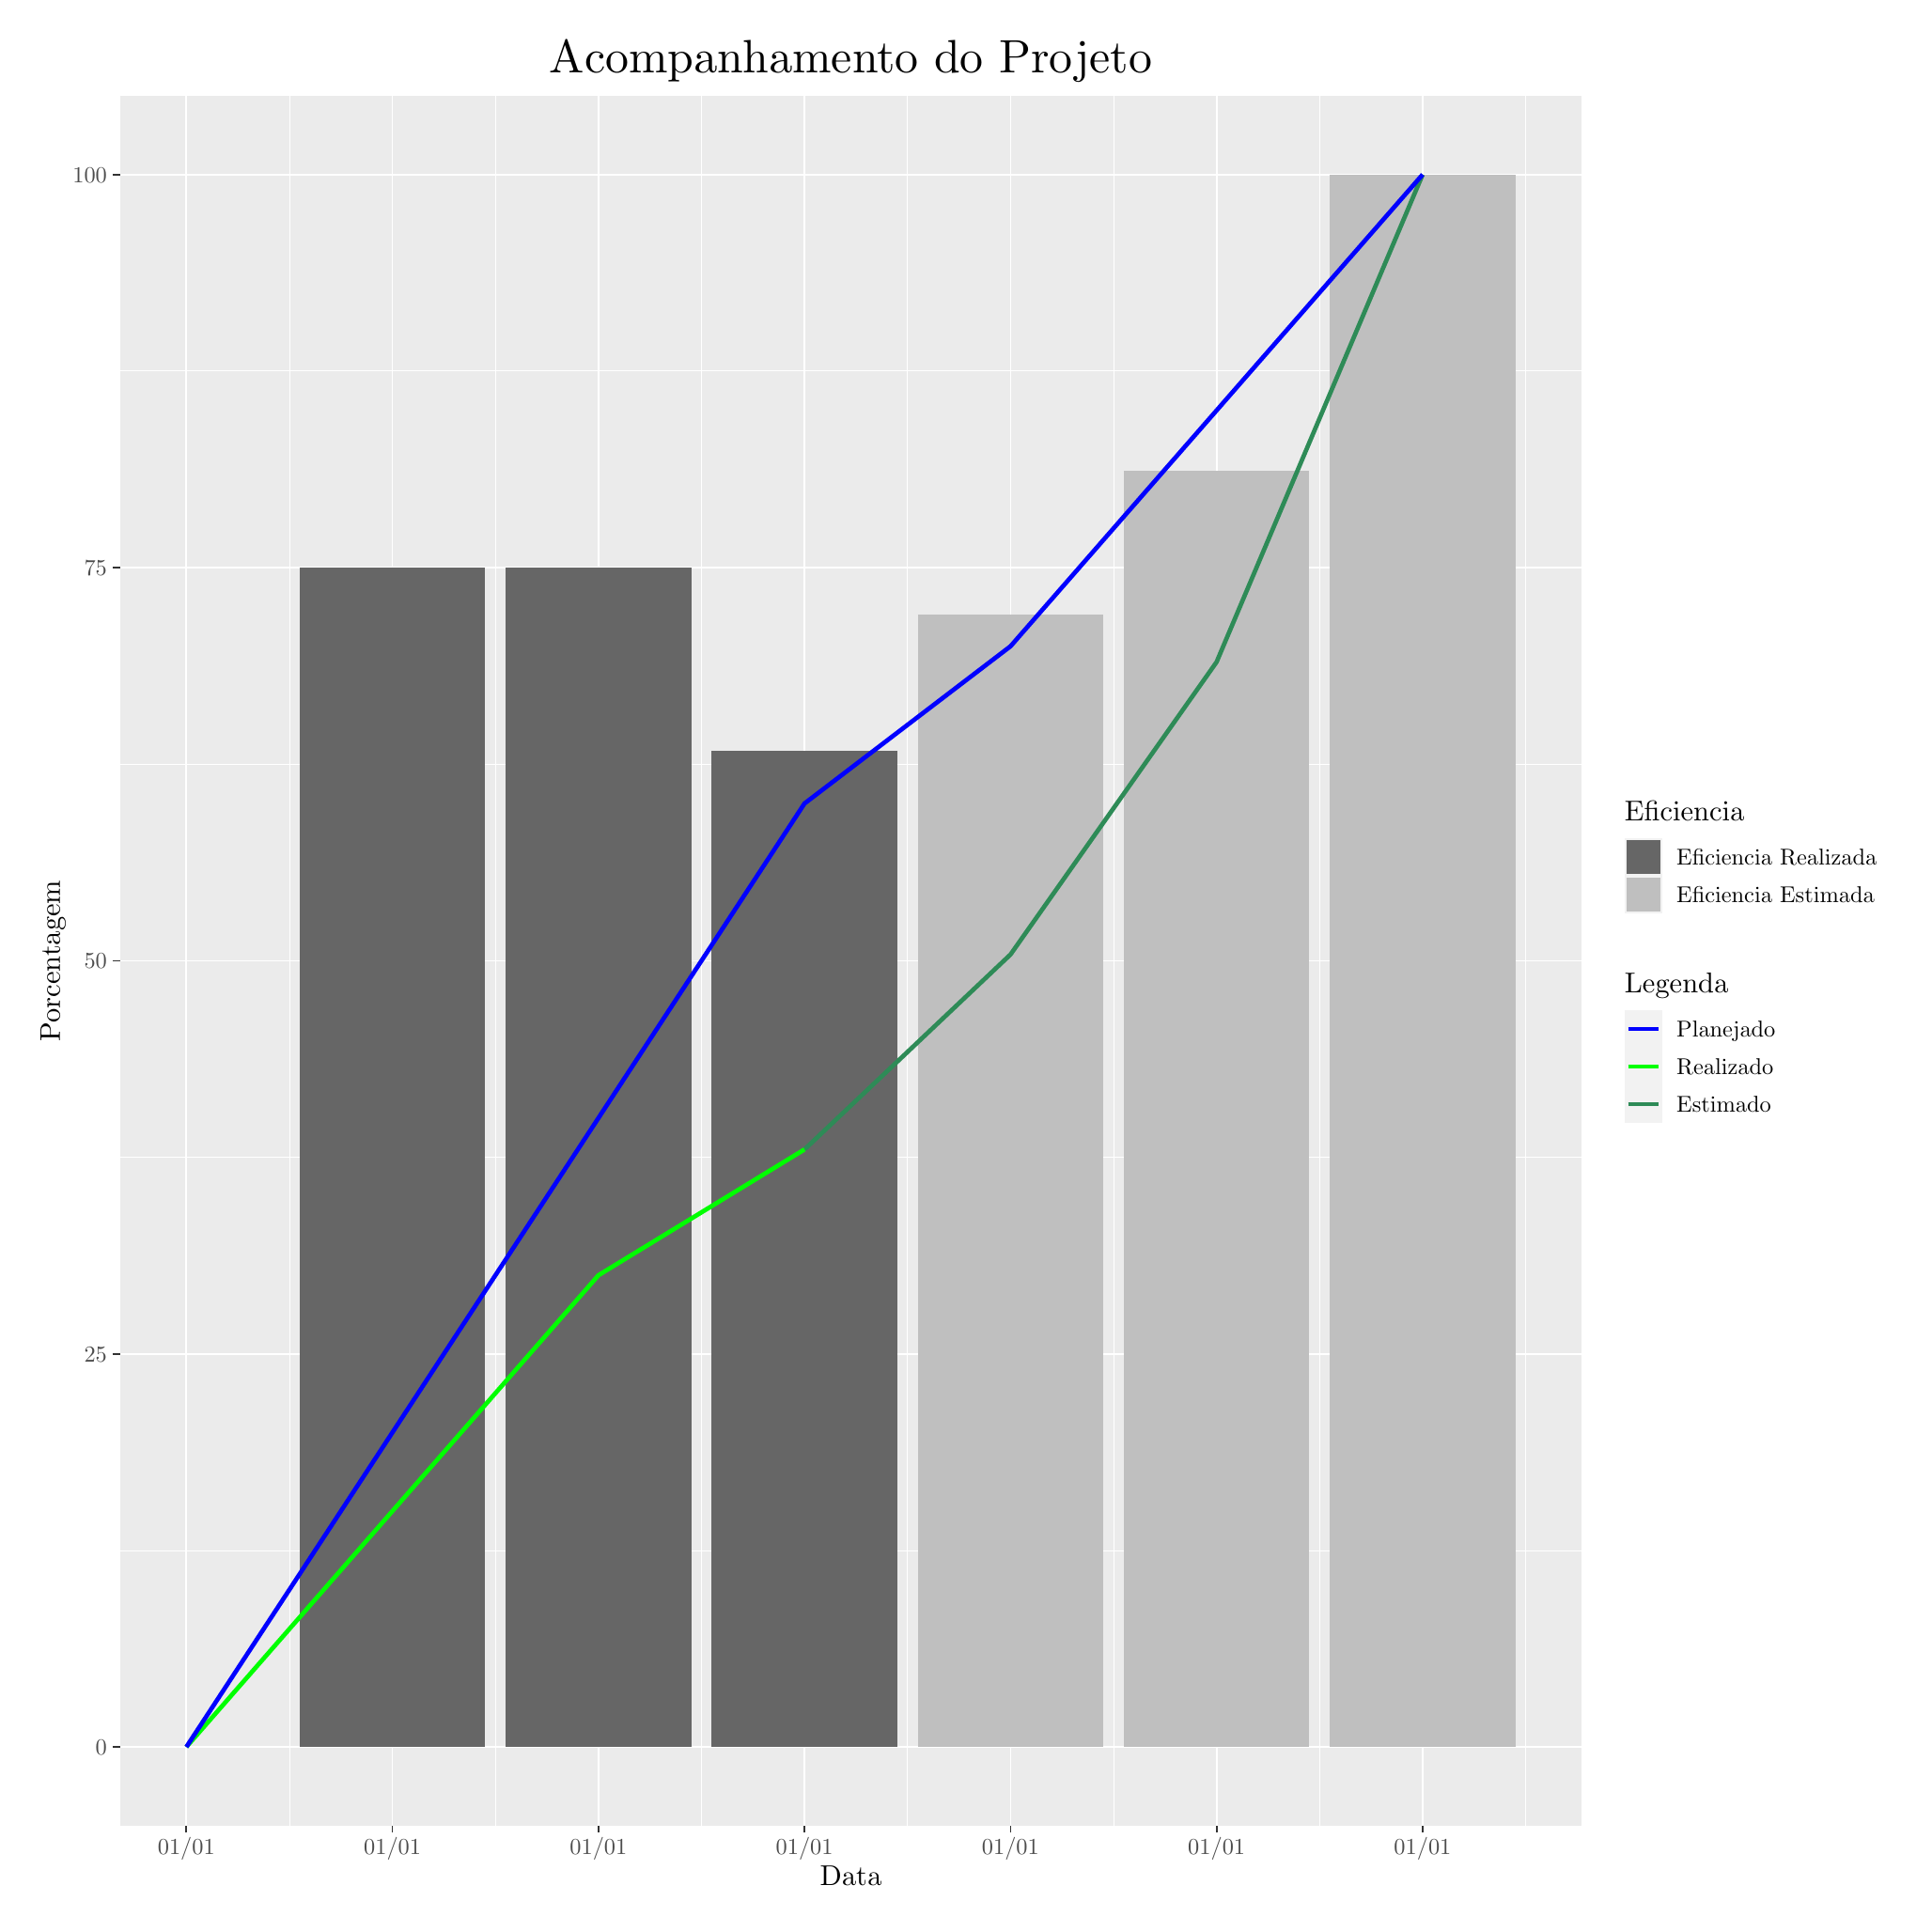
\begin{tikzpicture}[x=1pt,y=1pt]
\definecolor{fillColor}{RGB}{255,255,255}
\path[use as bounding box,fill=fillColor,fill opacity=0.00] (0,0) rectangle (722.70,722.70);
\begin{scope}
\path[clip] (  0.00,  0.00) rectangle (722.70,722.70);
\definecolor{drawColor}{RGB}{255,255,255}
\definecolor{fillColor}{RGB}{255,255,255}

\path[draw=drawColor,line width= 0.6pt,line join=round,line cap=round,fill=fillColor] (  0.00,  0.00) rectangle (722.70,722.70);
\end{scope}
\begin{scope}
\path[clip] ( 36.11, 30.69) rectangle (598.26,695.80);
\definecolor{fillColor}{gray}{0.92}

\path[fill=fillColor] ( 36.11, 30.69) rectangle (598.26,695.80);
\definecolor{drawColor}{RGB}{255,255,255}

\path[draw=drawColor,line width= 0.3pt,line join=round] ( 36.11,136.50) --
	(598.26,136.50);

\path[draw=drawColor,line width= 0.3pt,line join=round] ( 36.11,287.66) --
	(598.26,287.66);

\path[draw=drawColor,line width= 0.3pt,line join=round] ( 36.11,438.83) --
	(598.26,438.83);

\path[draw=drawColor,line width= 0.3pt,line join=round] ( 36.11,589.99) --
	(598.26,589.99);

\path[draw=drawColor,line width= 0.3pt,line join=round] (101.28, 30.69) --
	(101.28,695.80);

\path[draw=drawColor,line width= 0.3pt,line join=round] (180.51, 30.69) --
	(180.51,695.80);

\path[draw=drawColor,line width= 0.3pt,line join=round] (259.74, 30.69) --
	(259.74,695.80);

\path[draw=drawColor,line width= 0.3pt,line join=round] (338.98, 30.69) --
	(338.98,695.80);

\path[draw=drawColor,line width= 0.3pt,line join=round] (418.21, 30.69) --
	(418.21,695.80);

\path[draw=drawColor,line width= 0.3pt,line join=round] (497.44, 30.69) --
	(497.44,695.80);

\path[draw=drawColor,line width= 0.3pt,line join=round] (576.67, 30.69) --
	(576.67,695.80);

\path[draw=drawColor,line width= 0.6pt,line join=round] ( 36.11, 60.92) --
	(598.26, 60.92);

\path[draw=drawColor,line width= 0.6pt,line join=round] ( 36.11,212.08) --
	(598.26,212.08);

\path[draw=drawColor,line width= 0.6pt,line join=round] ( 36.11,363.24) --
	(598.26,363.24);

\path[draw=drawColor,line width= 0.6pt,line join=round] ( 36.11,514.41) --
	(598.26,514.41);

\path[draw=drawColor,line width= 0.6pt,line join=round] ( 36.11,665.57) --
	(598.26,665.57);

\path[draw=drawColor,line width= 0.6pt,line join=round] ( 61.66, 30.69) --
	( 61.66,695.80);

\path[draw=drawColor,line width= 0.6pt,line join=round] (140.90, 30.69) --
	(140.90,695.80);

\path[draw=drawColor,line width= 0.6pt,line join=round] (220.13, 30.69) --
	(220.13,695.80);

\path[draw=drawColor,line width= 0.6pt,line join=round] (299.36, 30.69) --
	(299.36,695.80);

\path[draw=drawColor,line width= 0.6pt,line join=round] (378.59, 30.69) --
	(378.59,695.80);

\path[draw=drawColor,line width= 0.6pt,line join=round] (457.83, 30.69) --
	(457.83,695.80);

\path[draw=drawColor,line width= 0.6pt,line join=round] (537.06, 30.69) --
	(537.06,695.80);
\definecolor{fillColor}{gray}{0.40}

\path[fill=fillColor] (105.24, 60.92) rectangle (176.55,514.41);

\path[fill=fillColor] (184.47, 60.92) rectangle (255.78,514.41);

\path[fill=fillColor] (263.71, 60.92) rectangle (335.02,443.87);
\definecolor{fillColor}{gray}{0.75}

\path[fill=fillColor] (342.94, 60.92) rectangle (414.25,496.27);

\path[fill=fillColor] (422.17, 60.92) rectangle (493.48,551.75);

\path[fill=fillColor] (501.40, 60.92) rectangle (572.71,665.57);
\definecolor{drawColor}{RGB}{46,139,87}

\path[draw=drawColor,line width= 1.7pt,line join=round] (299.36,290.69) --
	(378.59,365.66) --
	(457.83,478.13) --
	(537.06,665.57);
\definecolor{drawColor}{RGB}{0,255,0}

\path[draw=drawColor,line width= 1.7pt,line join=round] ( 61.66, 60.92) --
	(140.90,151.62) --
	(220.13,242.31) --
	(299.36,290.69);
\definecolor{drawColor}{RGB}{0,0,255}

\path[draw=drawColor,line width= 1.7pt,line join=round] ( 61.66, 60.92) --
	(140.90,181.85) --
	(220.13,302.78) --
	(299.36,423.71) --
	(378.59,484.18) --
	(457.83,574.87) --
	(537.06,665.57);
\end{scope}
\begin{scope}
\path[clip] (  0.00,  0.00) rectangle (722.70,722.70);
\definecolor{drawColor}{gray}{0.30}

\node[text=drawColor,anchor=base east,inner sep=0pt, outer sep=0pt, scale=  0.88] at ( 31.16, 57.89) {0};

\node[text=drawColor,anchor=base east,inner sep=0pt, outer sep=0pt, scale=  0.88] at ( 31.16,209.05) {25};

\node[text=drawColor,anchor=base east,inner sep=0pt, outer sep=0pt, scale=  0.88] at ( 31.16,360.21) {50};

\node[text=drawColor,anchor=base east,inner sep=0pt, outer sep=0pt, scale=  0.88] at ( 31.16,511.38) {75};

\node[text=drawColor,anchor=base east,inner sep=0pt, outer sep=0pt, scale=  0.88] at ( 31.16,662.54) {100};
\end{scope}
\begin{scope}
\path[clip] (  0.00,  0.00) rectangle (722.70,722.70);
\definecolor{drawColor}{gray}{0.20}

\path[draw=drawColor,line width= 0.6pt,line join=round] ( 33.36, 60.92) --
	( 36.11, 60.92);

\path[draw=drawColor,line width= 0.6pt,line join=round] ( 33.36,212.08) --
	( 36.11,212.08);

\path[draw=drawColor,line width= 0.6pt,line join=round] ( 33.36,363.24) --
	( 36.11,363.24);

\path[draw=drawColor,line width= 0.6pt,line join=round] ( 33.36,514.41) --
	( 36.11,514.41);

\path[draw=drawColor,line width= 0.6pt,line join=round] ( 33.36,665.57) --
	( 36.11,665.57);
\end{scope}
\begin{scope}
\path[clip] (  0.00,  0.00) rectangle (722.70,722.70);
\definecolor{drawColor}{gray}{0.20}

\path[draw=drawColor,line width= 0.6pt,line join=round] ( 61.66, 27.94) --
	( 61.66, 30.69);

\path[draw=drawColor,line width= 0.6pt,line join=round] (140.90, 27.94) --
	(140.90, 30.69);

\path[draw=drawColor,line width= 0.6pt,line join=round] (220.13, 27.94) --
	(220.13, 30.69);

\path[draw=drawColor,line width= 0.6pt,line join=round] (299.36, 27.94) --
	(299.36, 30.69);

\path[draw=drawColor,line width= 0.6pt,line join=round] (378.59, 27.94) --
	(378.59, 30.69);

\path[draw=drawColor,line width= 0.6pt,line join=round] (457.83, 27.94) --
	(457.83, 30.69);

\path[draw=drawColor,line width= 0.6pt,line join=round] (537.06, 27.94) --
	(537.06, 30.69);
\end{scope}
\begin{scope}
\path[clip] (  0.00,  0.00) rectangle (722.70,722.70);
\definecolor{drawColor}{gray}{0.30}

\node[text=drawColor,anchor=base,inner sep=0pt, outer sep=0pt, scale=  0.88] at ( 61.66, 19.68) {01/01};

\node[text=drawColor,anchor=base,inner sep=0pt, outer sep=0pt, scale=  0.88] at (140.90, 19.68) {01/01};

\node[text=drawColor,anchor=base,inner sep=0pt, outer sep=0pt, scale=  0.88] at (220.13, 19.68) {01/01};

\node[text=drawColor,anchor=base,inner sep=0pt, outer sep=0pt, scale=  0.88] at (299.36, 19.68) {01/01};

\node[text=drawColor,anchor=base,inner sep=0pt, outer sep=0pt, scale=  0.88] at (378.59, 19.68) {01/01};

\node[text=drawColor,anchor=base,inner sep=0pt, outer sep=0pt, scale=  0.88] at (457.83, 19.68) {01/01};

\node[text=drawColor,anchor=base,inner sep=0pt, outer sep=0pt, scale=  0.88] at (537.06, 19.68) {01/01};
\end{scope}
\begin{scope}
\path[clip] (  0.00,  0.00) rectangle (722.70,722.70);
\definecolor{drawColor}{RGB}{0,0,0}

\node[text=drawColor,anchor=base,inner sep=0pt, outer sep=0pt, scale=  1.10] at (317.19,  7.64) {Data};
\end{scope}
\begin{scope}
\path[clip] (  0.00,  0.00) rectangle (722.70,722.70);
\definecolor{drawColor}{RGB}{0,0,0}

\node[text=drawColor,rotate= 90.00,anchor=base,inner sep=0pt, outer sep=0pt, scale=  1.10] at ( 13.08,363.24) {Porcentagem};
\end{scope}
\begin{scope}
\path[clip] (  0.00,  0.00) rectangle (722.70,722.70);
\definecolor{fillColor}{RGB}{255,255,255}

\path[fill=fillColor] (609.26,375.97) rectangle (717.20,431.09);
\end{scope}
\begin{scope}
\path[clip] (  0.00,  0.00) rectangle (722.70,722.70);
\definecolor{drawColor}{RGB}{0,0,0}

\node[text=drawColor,anchor=base west,inner sep=0pt, outer sep=0pt, scale=  1.10] at (614.76,416.95) {Eficiencia};
\end{scope}
\begin{scope}
\path[clip] (  0.00,  0.00) rectangle (722.70,722.70);
\definecolor{fillColor}{gray}{0.95}

\path[fill=fillColor] (614.76,395.93) rectangle (629.22,410.38);
\end{scope}
\begin{scope}
\path[clip] (  0.00,  0.00) rectangle (722.70,722.70);
\definecolor{fillColor}{gray}{0.40}

\path[fill=fillColor] (615.48,396.64) rectangle (628.51,409.67);
\end{scope}
\begin{scope}
\path[clip] (  0.00,  0.00) rectangle (722.70,722.70);
\definecolor{fillColor}{gray}{0.40}

\path[fill=fillColor] (615.48,396.64) rectangle (628.51,409.67);
\end{scope}
\begin{scope}
\path[clip] (  0.00,  0.00) rectangle (722.70,722.70);
\definecolor{fillColor}{gray}{0.95}

\path[fill=fillColor] (614.76,381.47) rectangle (629.22,395.93);
\end{scope}
\begin{scope}
\path[clip] (  0.00,  0.00) rectangle (722.70,722.70);
\definecolor{fillColor}{gray}{0.75}

\path[fill=fillColor] (615.48,382.18) rectangle (628.51,395.21);
\end{scope}
\begin{scope}
\path[clip] (  0.00,  0.00) rectangle (722.70,722.70);
\definecolor{fillColor}{gray}{0.75}

\path[fill=fillColor] (615.48,382.18) rectangle (628.51,395.21);
\end{scope}
\begin{scope}
\path[clip] (  0.00,  0.00) rectangle (722.70,722.70);
\definecolor{drawColor}{RGB}{0,0,0}

\node[text=drawColor,anchor=base west,inner sep=0pt, outer sep=0pt, scale=  0.88] at (634.72,400.12) {Eficiencia Realizada};
\end{scope}
\begin{scope}
\path[clip] (  0.00,  0.00) rectangle (722.70,722.70);
\definecolor{drawColor}{RGB}{0,0,0}

\node[text=drawColor,anchor=base west,inner sep=0pt, outer sep=0pt, scale=  0.88] at (634.72,385.67) {Eficiencia Estimada};
\end{scope}
\begin{scope}
\path[clip] (  0.00,  0.00) rectangle (722.70,722.70);
\definecolor{fillColor}{RGB}{255,255,255}

\path[fill=fillColor] (609.26,295.40) rectangle (678.22,364.97);
\end{scope}
\begin{scope}
\path[clip] (  0.00,  0.00) rectangle (722.70,722.70);
\definecolor{drawColor}{RGB}{0,0,0}

\node[text=drawColor,anchor=base west,inner sep=0pt, outer sep=0pt, scale=  1.10] at (614.76,350.83) {Legenda};
\end{scope}
\begin{scope}
\path[clip] (  0.00,  0.00) rectangle (722.70,722.70);
\definecolor{fillColor}{gray}{0.95}

\path[fill=fillColor] (614.76,329.80) rectangle (629.22,344.26);
\end{scope}
\begin{scope}
\path[clip] (  0.00,  0.00) rectangle (722.70,722.70);
\definecolor{drawColor}{RGB}{0,0,255}

\path[draw=drawColor,line width= 1.7pt,line join=round] (616.21,337.03) -- (627.77,337.03);
\end{scope}
\begin{scope}
\path[clip] (  0.00,  0.00) rectangle (722.70,722.70);
\definecolor{drawColor}{RGB}{0,0,255}

\path[draw=drawColor,line width= 1.7pt,line join=round] (616.21,337.03) -- (627.77,337.03);
\end{scope}
\begin{scope}
\path[clip] (  0.00,  0.00) rectangle (722.70,722.70);
\definecolor{drawColor}{RGB}{0,0,255}

\path[draw=drawColor,line width= 1.7pt,line join=round] (616.21,337.03) -- (627.77,337.03);
\end{scope}
\begin{scope}
\path[clip] (  0.00,  0.00) rectangle (722.70,722.70);
\definecolor{fillColor}{gray}{0.95}

\path[fill=fillColor] (614.76,315.35) rectangle (629.22,329.80);
\end{scope}
\begin{scope}
\path[clip] (  0.00,  0.00) rectangle (722.70,722.70);
\definecolor{drawColor}{RGB}{0,255,0}

\path[draw=drawColor,line width= 1.7pt,line join=round] (616.21,322.58) -- (627.77,322.58);
\end{scope}
\begin{scope}
\path[clip] (  0.00,  0.00) rectangle (722.70,722.70);
\definecolor{drawColor}{RGB}{0,255,0}

\path[draw=drawColor,line width= 1.7pt,line join=round] (616.21,322.58) -- (627.77,322.58);
\end{scope}
\begin{scope}
\path[clip] (  0.00,  0.00) rectangle (722.70,722.70);
\definecolor{drawColor}{RGB}{0,255,0}

\path[draw=drawColor,line width= 1.7pt,line join=round] (616.21,322.58) -- (627.77,322.58);
\end{scope}
\begin{scope}
\path[clip] (  0.00,  0.00) rectangle (722.70,722.70);
\definecolor{fillColor}{gray}{0.95}

\path[fill=fillColor] (614.76,300.90) rectangle (629.22,315.35);
\end{scope}
\begin{scope}
\path[clip] (  0.00,  0.00) rectangle (722.70,722.70);
\definecolor{drawColor}{RGB}{46,139,87}

\path[draw=drawColor,line width= 1.7pt,line join=round] (616.21,308.12) -- (627.77,308.12);
\end{scope}
\begin{scope}
\path[clip] (  0.00,  0.00) rectangle (722.70,722.70);
\definecolor{drawColor}{RGB}{46,139,87}

\path[draw=drawColor,line width= 1.7pt,line join=round] (616.21,308.12) -- (627.77,308.12);
\end{scope}
\begin{scope}
\path[clip] (  0.00,  0.00) rectangle (722.70,722.70);
\definecolor{drawColor}{RGB}{46,139,87}

\path[draw=drawColor,line width= 1.7pt,line join=round] (616.21,308.12) -- (627.77,308.12);
\end{scope}
\begin{scope}
\path[clip] (  0.00,  0.00) rectangle (722.70,722.70);
\definecolor{drawColor}{RGB}{0,0,0}

\node[text=drawColor,anchor=base west,inner sep=0pt, outer sep=0pt, scale=  0.88] at (634.72,334.00) {Planejado};
\end{scope}
\begin{scope}
\path[clip] (  0.00,  0.00) rectangle (722.70,722.70);
\definecolor{drawColor}{RGB}{0,0,0}

\node[text=drawColor,anchor=base west,inner sep=0pt, outer sep=0pt, scale=  0.88] at (634.72,319.55) {Realizado};
\end{scope}
\begin{scope}
\path[clip] (  0.00,  0.00) rectangle (722.70,722.70);
\definecolor{drawColor}{RGB}{0,0,0}

\node[text=drawColor,anchor=base west,inner sep=0pt, outer sep=0pt, scale=  0.88] at (634.72,305.09) {Estimado};
\end{scope}
\begin{scope}
\path[clip] (  0.00,  0.00) rectangle (722.70,722.70);
\definecolor{drawColor}{RGB}{0,0,0}

\node[text=drawColor,anchor=base,inner sep=0pt, outer sep=0pt, scale=  1.80] at (317.19,704.80) {Acompanhamento do Projeto};
\end{scope}
\end{tikzpicture}
